% 2010 年福建卷理科第 6 题：长方体 ABCD-A1B1C1D1 被平面 EFGH 截去几何体 EFGHB1C1。
% 来源 PDF：普通高考/2010/2010福建理.pdf，SHA-256 7c811af1fc113435bb53b4e967c30d769e6297a558f617dd322adf3152d9df84。
% 原页：第 1 页（A3 三栏）第 2 栏上部，书页码 589。
% 重绘依据：照原页斜二测画法，前面 ABB1A1 为矩形、后底面按右上方向平移；
%   E 在棱 A1B1 上、H 在棱 D1C1 上且 EH∥A1D1；F 在棱 BB1 上、G 在棱 CC1 上，F 与 G 等高。
%   实线为可见棱及截面 EFGH 的边；虚线为被截面遮挡的棱 A1B1 上 E 到 B1 段、B1F、B1C1、C1H、C1G
%   与底面、后棱；灰色平行四边形为截面 EFGH。
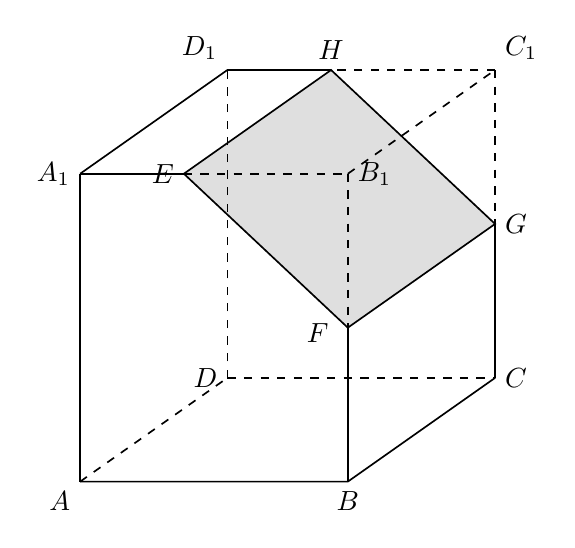
\begin{tikzpicture}[scale=0.85, semithick]
  \coordinate (A)  at (0,0);
  \coordinate (B)  at (4,0);
  \coordinate (C)  at (6.2,1.55);
  \coordinate (D)  at (2.2,1.55);
  \coordinate (A1) at (0,4.6);
  \coordinate (B1) at (4,4.6);
  \coordinate (C1) at (6.2,6.15);
  \coordinate (D1) at (2.2,6.15);
  \coordinate (E)  at (1.55,4.6);
  \coordinate (H)  at (3.75,6.15);
  \coordinate (F)  at (4,2.3);
  \coordinate (G)  at (6.2,3.85);

  % 截面 EFGH
  \fill[gray!25] (E) -- (F) -- (G) -- (H) -- cycle;

  % 可见棱
  \draw (A) -- (B) -- (C);
  \draw (C) -- (G);
  \draw (A) -- (A1);
  \draw (A1) -- (D1);
  \draw (D1) -- (H);
  \draw (A1) -- (E);
  \draw (B) -- (F);
  % 截面边界
  \draw (E) -- (F) -- (G) -- (H) -- cycle;

  % 被遮挡的棱
  \draw[dashed] (A) -- (D);
  \draw[dashed] (D) -- (C);
  \draw[dashed] (D) -- (D1);
  \draw[dashed] (E) -- (B1);
  \draw[dashed] (B1) -- (F);
  \draw[dashed] (B1) -- (C1);
  \draw[dashed] (C1) -- (H);
  \draw[dashed] (C1) -- (G);

  \node[below left]  at (A)  {$A$};
  \node[below]       at (B)  {$B$};
  \node[right]       at (C)  {$C$};
  \node[left]        at (D)  {$D$};
  \node[left]        at (A1) {$A_1$};
  \node[right]       at (B1) {$B_1$};
  \node[above right] at (C1) {$C_1$};
  \node[above left]  at (D1) {$D_1$};
  \node[left]        at (E)  {$E$};
  \node[above]       at (H)  {$H$};
  \node[left]        at (3.86,2.22) {$F$};
  \node[right]       at (G)  {$G$};
\end{tikzpicture}
